%%%%%%%%%%%%%%%%%%%%%%%%%%%%%%%%%%%%%%%%%%%%%%%%%%%%%%%%%%%%%%%%%%%%%%%%%%%%%%%%
%2345678901234567890123456789012345678901234567890123456789012345678901234567890
%        1         2         3         4         5         6         7         8

\documentclass[letterpaper, 10 pt, conference]{ieeeconf}  % Comment this line out if you need a4paper

%\documentclass[a4paper, 10pt, conference]{ieeeconf}      % Use this line for a4 paper

\IEEEoverridecommandlockouts                              % This command is only needed if
                                                          % you want to use the \thanks command

\overrideIEEEmargins                                      % Needed to meet printer requirements.

% See the \addtolength command later in the file to balance the column lengths
% on the last page of the document

% The following packages can be found on http:\\www.ctan.org
%\usepackage{graphics} % for pdf, bitmapped graphics files
\usepackage{graphicx}
\newcommand{\squeezeup}{\vspace{-1.0mm}}
%\usepackage{epsfig} % for postscript graphics files
%\usepackage{mathptmx} % assumes new font selection scheme installed
%\usepackage{times} % assumes new font selection scheme installed
%\usepackage{amsmath} % assumes amsmath package installed
%\usepackage{amssymb}  % assumes amsmath package installed

\title{\LARGE \bf
Software Architecture for Validation and Verification of Cooperative Autonomy of Multiple Thermaling Gliders* }

\author{Dmitrij Koniajev$^{1}$, Vladimir Fedorov$^{2}$ \\
    Nahum Camacho$^{3}$, Vladimir Dobrokhodov$^{4}$, and Kevin Jones$^{5}$% <-this % stops a space
\thanks{*The project has been supported over the last 3 years by a number of
sponsors including the NPS Consortium for Robotics and Unmanned Systems Education and Research, the Army Research Lab, and "The Multidisciplinary Studies Support for USMC Expeditionary Energy Office."}% <-this % stops a space
\thanks{$^{1}$Senior developer in the Demand-Side Platform team,
        Adform Lithuania, J. Jasinskio 16C, LT-01112 Vilnius, Lithuania,
        {\tt\small {dimchansky@gmail.com}}}%
\thanks{$^{2}$Postdoctoral researcher at the Department of Wind Energy,
        Technical University of Denmark, Building 114, Frederiksborgvej 399, DK-4000 Roskilde,
        Denmark
        {\tt\small {vlfe@dtu.dk}}}%
\thanks{$^{3-5}$authors are with the Department of Mechanical and Aerospace Engineering,
        Naval Postgraduate School, Monterey, CA 93943, USA
        {\tt\small {ncamacho, vldobr, jones}@nps.edu}}%
} % end of author

\begin{document}

\maketitle \thispagestyle{empty} \pagestyle{empty}


%%%%%%%%%%%%%%%%%%%%%%%%%%%%%%%%%%%%%%%%%%%%%%%%%%%%%%%%%%%%%%%%%%%%%%%%%%%%%%%%
\begin{abstract}
This paper describes the evolutionary steps in the design of cooperative control capability of multiple autonomous soaring gliders. The paper presents the envisioned concept of operation and reviews the principal components necessary to enable the ''eternal`` flight of a fleet of gliders. The paper then focuses on the design of the software architecture that allows to verify the designed control algorithms in a high-fidelity simulation prior to the actual flight. The software architecture is based on the tight integration of Condor soaring flight simulator with the advanced capabilities of MatLab/Simulink design environment. The key benefits of the software for the flight control system design include the ability to realistically represent the atmospheric convective airflow and its interaction with 3D terrain, the high-fidelity flight dynamics of a variety of soaring gliders, and the advance MathWorks' tools of the control development and flight data analysis. The cooperative capability is implemented by communicating the states of multiple gliders over the network. Ultimately, the developed system allows verification and validation of advanced cooperative control strategies and their comparison against best practices of human piloted soaring flight.
\end{abstract}


%%%%%%%%%%%%%%%%%%%%%%%%%%%%%%%%%%%%%%%%%%%%%%%%%%%%%%%%%%%%%%%%%%%%%%%%%%%%%%%%
\section{INTRODUCTION}
\squeezeup
Imagine a large team of gracefully soaring autonomous gliders, instrumented with sensors capable of detecting convective air currents in the environment. The gliders are launched from a remote location and assigned to provide, for example, wide area network coverage or to serve as pseudo Low-Earth-Orbit satellites to aid in fighting forest fires or to support border protection. The gliders reach the area of operation and remain there unattended for an extended period of time, perhaps up to a year. When a need for maintenance arises, the distributed intelligent algorithm reconfigures the team of gliders and calls back the aircraft in need of service. In turn, when a substitute or serviced aircraft returns, the same algorithm reconfigures the team to accept the new player. Members of the flock can either operate in a distributed fashion or fly together in a suitable formation to provide a more focused capability. The latter may include cooperative distributed sensing to achieve a desired sensor resolution, tracking of weather formations, border patrol, and many other tasks that are currently provided by much larger, heavier, and more expensive systems.

There have been several projects that have sought to capitalize on convective lift and solar photovoltaic energy in the environment to offset or remove the need for propulsion. First demonstrated by human pilots in 1900s \cite{Simons:1998}, the idea of soaring in convective air became feasible for onboard autonomous implementation only in the 1990s, see \cite{Wharington:1998}. A challenge for these vehicles revolves around locating the regions of advantageous lift. While enabling the desired functionality by primarily mimicking the birds flight and indeed achieving significant extended flight capabilities, see \cite{Edwards:2008,Allen:2006,Allen:2007}, most of the algorithms used heuristics in the identification of the updraft strength, its potential utility in energy gain, and the decision of when and how to enter the updraft. The reason for employing heuristic approaches is obvious, since the strength of the updraft and its efficiency are both subject to significant uncertainties and are hard to formalize. The most recent development by~\cite{AKlass_CDC:2012,AKlass_JGCD:2012} demonstrated that teaming aircraft working cooperatively could improve the probability of successful detection and exploitation of thermals by splitting up the search task and sharing location data for regions of lift. Combining the ability to exploit natural lift in the environment with photo-voltaic or wind-driven energy production, the vehicles should be able to stay aloft $24/7$, while still having enough additional energy to support the weight and power of meaningful payloads.


\section{Integrated Control Development Environment}

\subsection{Key Enablers of Cooperative Autonomy}

Development of the collaborative capability is based on an assumption that single glider has an onboard autopilot (AP). In the soaring glider case, the AP provides the typical for UAVs stability, guidance and navigation capabilities, however with the energy management algorithms reflecting the absence of traditional propulsion. The need for multiple UAVs arises because an autonomous glider first needs to find a thermal (the area of convective air), and therefore acts as a sensor of thermals that cannot be remotely detected by the onboard sensors. A thermal can only be sensed when the glider approaches it, therefore the effectiveness of the soaring flight directly depends on the rate of detection of thermals. The detection rate can be increased~\cite{AKlass_JGCD:2012} by utilizing multiple gliders that fly in a given air volume and share information about their findings.

Therefore, in order to enable the collaborative flight of autonomous thermal soaring gliders, it is envisioned that each glider is equipped with online algorithms of convective thermals search, detection, and exploitation, as well as the collaborative decision making and communication methods; see the concept of collaborative flight in Figure.\ref{fig:coop_scheme}.
%%%%%%%%%%
\begin{figure}[thpb]
  \centering
  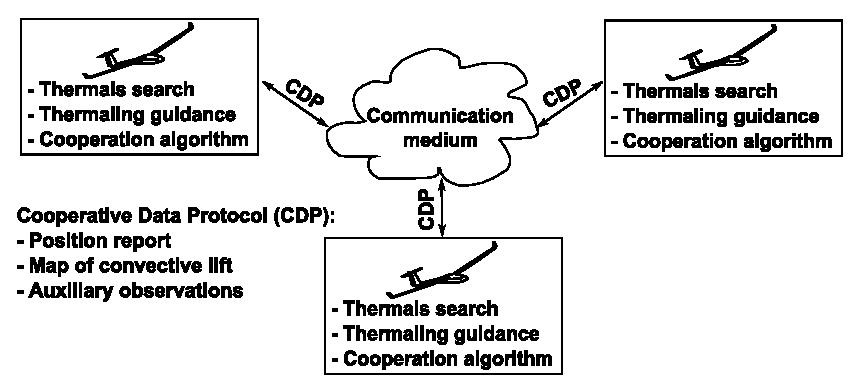
\includegraphics[scale=0.5]{Figures/coop_scheme_small.eps}
  \caption{Cooperation of autonomous gliders.}
  \label{fig:coop_scheme}
\end{figure}
%%%%%%%%%%
\squeezeup
The algorithms will run online to identify the inherent flight dynamics of the glider, which are used to detect the thermal updrafts. When flying in the updraft, the thermaling guidance algorithm is engaged to enable the maximum energy harvesting efficiency of the updraft’s free energy. On the other hand it estimates the updraft geometry and motion that are used to georeference the updraft, and share its utility properties (strength) across the network of collaborative gliders. Finally, the distributed knowledge about the existing updrafts needs to be intelligently utilized to maximize the benefit of the team of gliders flying with a specific operational objective.

\subsection{Architecture of High-fidelity Control Design Environment}
\squeezeup
It is clear from the preceding discussion that the desired set of enabling algorithms is significant and includes formalized knowledge from various disciplines including the flight dynamics, flight control, aerodynamics, meteorology, orography, etc. First to be developed is the high fidelity glider dynamics. Next, an advanced autopilot capable of thermals detection and autonomous soaring is to be designed and put into control of a free flying glider. A realistic weather model, including both the vertical air movements and small-scale turbulence models, has to be implemented within a considered scale of operational region. All this is to be augmented by the distributed cooperation algorithm and the communication model that both account for the distributed nature of cooperation and possibly significant losses in communication. Clearly, that even the development of high-fidelity flight dynamics of soaring glider and the realistic weather models represents a significant effort by itself. On the other hand, to verify the efficiency of the developed algorithms a number of flight tests needs to be performed. Thus,  recognizing the value of flight testing and still accounting for the complexity of flight experimentation, the project builds a high-fidelity numerical simulation and control design environment that provides the convenience and rigor of control algorithm development. To this end, the project developed a realistic simulation environment that is based on tight integration of MatLab/Simulink \cite{MATLAB:2013} control design capabilities with the high-fidelity flight dynamics and atmospheric effects of the Condor soaring simulator, see \cite{Condor:2013:Online}.


Condor Soaring Simulator (Condor) is a Microsoft Windows application developed around a decade ago. It is a very well-known soaring flight simulator within the glider pilot community around the globe. The Condor soaring simulator is one of the most realistic simulators compared to real life soaring; the software has been designed focusing on the fundamentals of aerodynamic flight, and the atmosphere and weather physics. Recognized also for the high realism of visualization, this simulator has been used by human glider pilots to acquire initial skills and to maintain their proficiency during off-season.
%The Condor allows to advance piloting skills in different wing loading conditions and weight balancing, %various flight regimes including stall and spin. Furthermore, the pilots can experience soaring flight %in different areas of the world, test their skills against other pilots in individual and team %competitions.
The key features of the Condor soaring simulator that are important enablers of the autonomous soaring are provided below, see \cite{Condor:2013:Online} for more details:
\squeezeup
\begin{itemize}
  \item advanced 6DOF \emph{flight dynamics} model run by real-time high-fidelity computational engine (up to 500 cycles per second); it includes the sailplane's \emph{damage simulation} with an account of the flutter, high $g-load$ stress, and aircraft collisions;
  \item accurate sailplane \emph{performance and handling qualities} including the flight at critical and beyond critical angles of attack;
  \item defines the \emph{weather model} with an outstanding level of details where such phenomena as convectional thermal updraft, slope updraft, ridge updraft, lee-side waves, exposure to sun that travels at side-real rate are simulated; for example, thermal updrafts reflect all phases of the real thermals including the formation, upraise and drifting with the wind, cloud forming, increase in power near the cloud base due to the condensation process in the cloud and finally the dissolving phase;
  \item the location and strength of thermals \emph{accounts for the ground features} like variable terrain (ridges and valleys), forests, swamps, fields, and man-made structures like cities and villages; wavelength depends on the wind speed and stability of the atmosphere;
  \item implements $3D$ \emph{isotropic turbulence model} for thermal convection and mechanical turbulence.
\end{itemize}
The simulator provides real-time output of the glider state vector, which is extremely useful for the present project. The output can be done using a serial RS232 serial interface or via UDP protocol. The possibility of on-line flights together with other glider pilots is one of the main advantages of the Condor simulator in application to the automation of the soaring flight.
%%%%%%%%%%
\begin{figure}[thpb]
  \centering
  \includegraphics[scale=0.3]{Figures/api_arch.eps}
  \caption{The Condor API architecture.}
  \label{fig:api_arch}
\end{figure}
%%%%%%%%%%
In order to harness the features of high-fidelity soaring simulation and connect them with advanced capabilities of control systems design provided by the MatLab/Simulink software, an unobtrusive and invisible for the original Condor software service has been developed. The key objective for this ``Condor API'' service is to provide low-level interoperability between the Simulink and Condor. This interoperability\footnote{EU Computer Program Directive~\cite{EU_CPD:2009:Online} and Sec. 103(f) of the DMCA (17 U.S.C. § 1201 (f))~\cite{DMCA:2013:Online} allow reverse engineering for the purposes of interoperability.} has been made possible by using reverse engineering without modifying any of the licensed software. Presented in Figure.\ref{fig:api_arch}, the Condor API service significantly extends the aircraft data, which Condor simulator streams to external applications. The data set includes parameters like the plane position, true airspeed, wind course, wind speed, MacCready setting, and the control surfaces deflection. The Condor API then streams the aircraft data to an external application using the UDP protocol. Utilizing this API, an external application can send the control surface commands back to the Condor API service via UDP, thus effectively establishing the software in the loop (SIL) environment, see Figure.\ref{fig:SIL}.
%%%%%%%%%%
\begin{figure}[thpb]
  \centering
  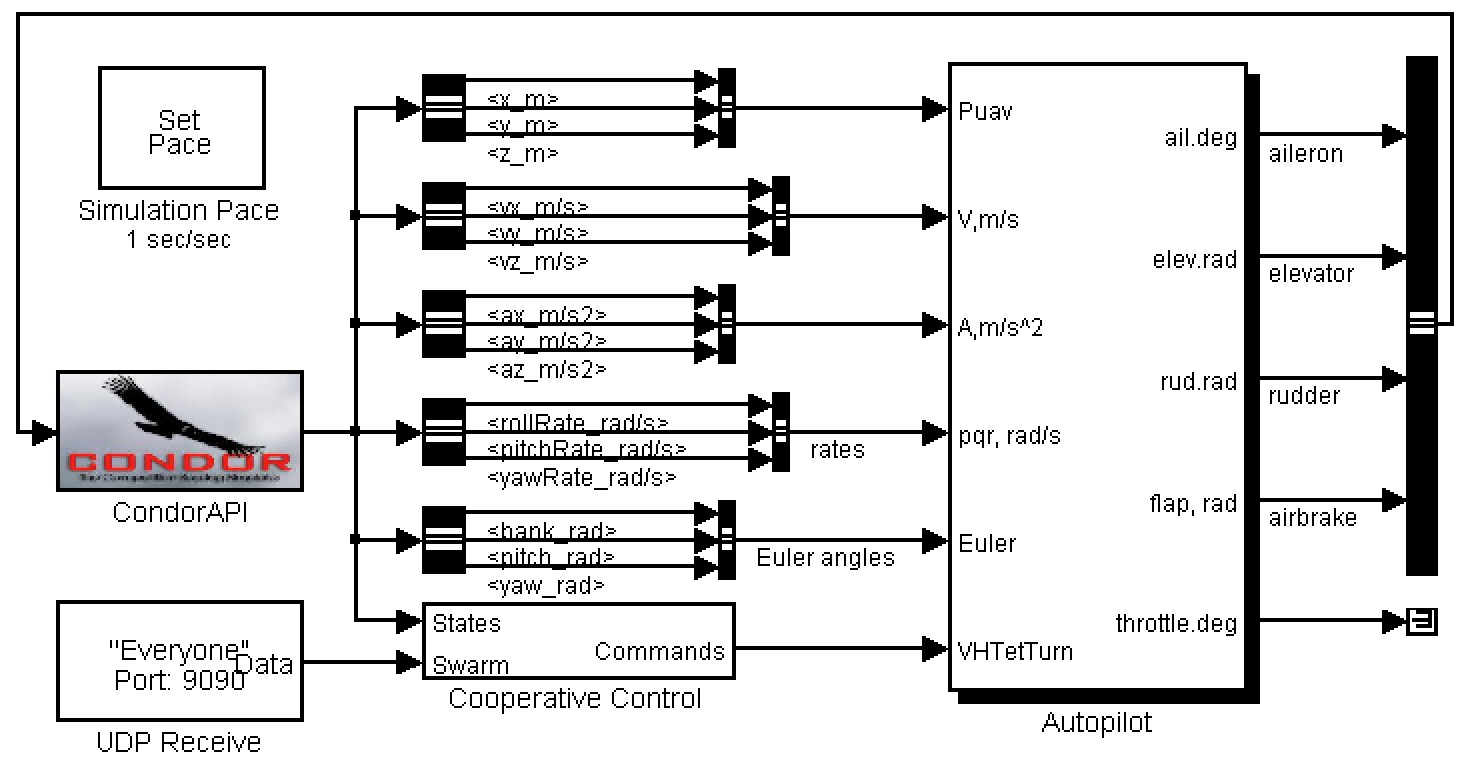
\includegraphics[scale=0.3]{Figures/SIL.eps}
  \caption{SIL environment integrates the capabilities of Simulink and Condor.}
  \label{fig:SIL}
\end{figure}
%%%%%%%%%%

Verification and validation (V\&V) of cooperative control strategies that take significant time to evolve in a distributed settings can be very difficult. To facilitate early identification of correct strategies and save time a visualization of cooperative strategies might be very effective. To this end, the Condor API service has been expanded with the ``FlightRadar'' external application that provides the capability to represent multiple evolving trajectories in one $3D$ map. To visualize the strategies of multiple competing soaring gliders in real-time the FlightRadar streams the telemetry information to Google Maps~\cite{GoogleMaps:2013:Online}, see an example of a half-hour flight in Figure.\ref{fig:FlightRadar}.
%%%%%%%%%%
\begin{figure}[thpb]
  \centering
  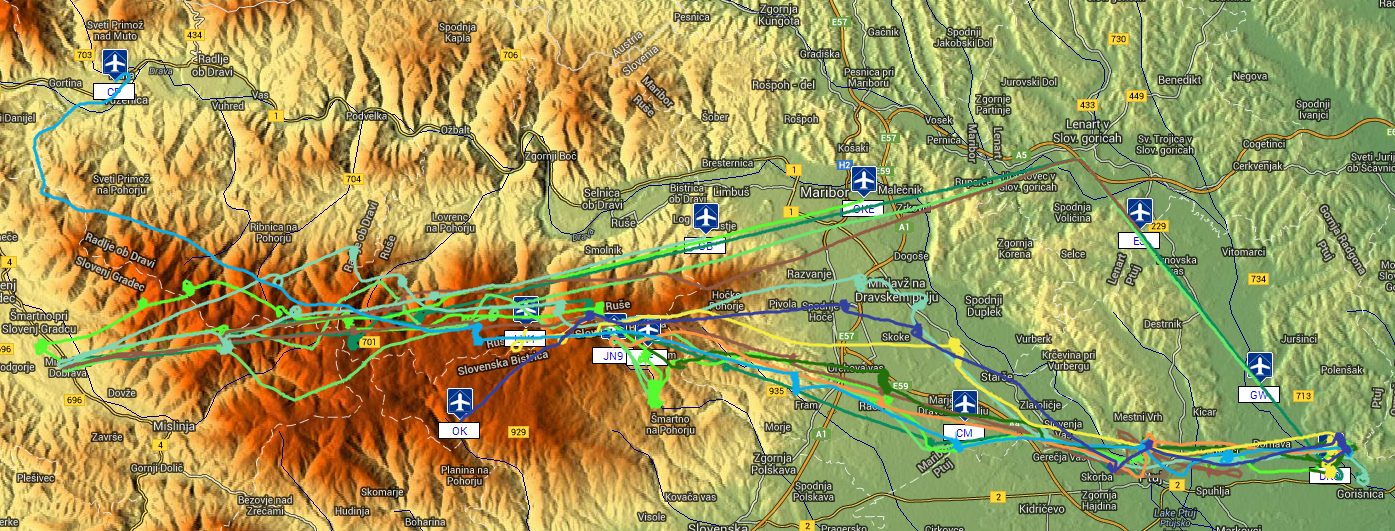
\includegraphics[scale=0.17]{Figures/flightradar_highlevel.eps}
  \caption{Evolution of cooperative strategies in Google Maps.}
  \label{fig:FlightRadar}
\end{figure}
%%%%%%%%%%

An example of possible setup for the design and V\&V of the cooperative soaring algorithms is given in Figure. \ref{fig:DevEnv} that represents a scenario where the autonomous gliders and the human pilots can fly together. Current weather conditions and interaction between the gliders in Condor simulator is handled by the Condor server application that can be deployed either in the same local network as the Condor Soaring Simulator or a dedicated Internet server provided by the company can be utilized; a set of servers is publicly available with their IP addresses and settings available to the registered users. A modelled glider communicates with the server via the Condor protocol over the Internet/network as in a typical computer game in multi-player mode. The Condor-Simulink SIL environment runs on the same (or a separate) computer and interacts via UDP protocol with the Condor API service. The multiple instances of Condor-Simulink SIL environments share knowledge among themselves via the cooperation protocol (CDP) within the local computer network. In addition, this setup also allows gliders to be controlled by human pilots operating within the same network by using the original Condor simulator client application.

\begin{figure}[thpb]
  \centering
  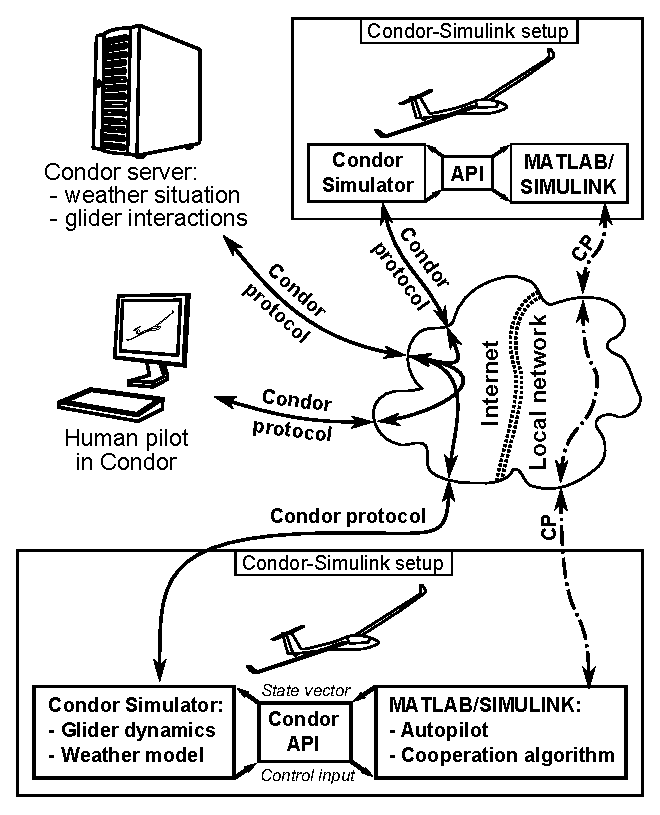
\includegraphics[scale=0.45]{Figures/dev_env_.eps}
  \caption{Possible setup of two SIL environments and a glider operated by a human pilot; Condor simulator server is running on a dedicated PC.}
  \label{fig:DevEnv}
\end{figure}

Harnessing the features of Condor soaring simulator allows leveraging the advanced capabilities of the MatLab/Simulink control design environment, thus resulting in a high-fidelity control design setup for cooperative soaring flight. Thus, the developed setup provides a convenient interface to researchers that allows them to quickly connect to the simulator and focus on the development of novel cooperative control.

\subsection{Potential Capabilities and Future Improvements}
\squeezeup
In the current implementation the intelligent agents, which are implemented by the Simulink model, share the states of a glider and its local onboard knowledge of thermaling convective lift via multicast UDP messages. This communication mechanism allows to run the Condor soaring simulator and Matlab/Simulink on different machines connected over the local network. As a result, this capability enables a competitive flight of multiple soaring gliders inside one local network. In turn, the availability of the multi-player mode in the Condor opens the possibilities for testing of cooperation algorithm of the unmanned gliders in the realistic environment, and validation of the algorithm against the behavior of a group of human pilots in a wide range of weather conditions.

At the same time the UDP communication has also its flaws. Since, in general, the UDP multicast (it is used to share the knowledge among gliders) over the Internet is not possible because the multicast packages are not routed, the cooperative competitive flight of multiple autonomous gliders placed in different networks is not possible; it is possible only inside one local network. Another limitation
is that multiple independent groups of autonomous agents located on the same local network at the same time can mislead each other.

The future version of the Condor API service could be improved by building a distributed Condor API system, which would consist of a number of Condor API services communicating with each other using gossip protocol\cite{Gupta:2006}. The distribution mechanism could be implemented using TCP/IP sockets like in the distributed Erlang systems \cite{Erlang:2013:Online} or Akka actors \cite{Akka:2013:Online}. This will solve the aforementioned problems and allow to create more powerful distributed agents.

\section{Principles of Convective Lift Detection and Cooperative Exploitation}
\squeezeup
To illustrate the utility of the developed SIL integrated environment a brief outline of the algorithms~\cite{AKlass_JGCD:2012} developed to enable the cooperative soaring is presented next.

The onboard algorithm of detecting a thermal is based on two complementary approaches. The first approach utilizes the inherent sink polar, and the second one is based on the total energy of the system. However, conceptually they are similar as they compare the natural metrics of the system with the same metrics actually measured in flight.

\emph{The sink polar} is the function of vertical sink rate versus the true airspeed (TAS) - of a particular glider can be practically achieved in extensive experimentation. Sink polars are roughly quadratic in nature, and a least-squares approach yields suitable coefficients based on the historical data. In the developed approach, the estimates of the sink-polar were first made by post-processing a collection of experimental flight results obtained in low-wind, low-lift conditions. Further in flight, a recursive linear least square estimator is used in real-time to account for specific variation in the platform and atmospheric conditions at that moment. The detection of a thermal and estimation of its intensity, that contributes to the recursive identification of its parameters, are based on comparison of the currently measured sink rate with the sink rate predicted by the polar for a measured TAS. If the measured sink rate is smaller than predicted, then there is a thermal.

\emph{The total energy} approach is based on the concept that the mechanical energy $E_{tot}$ of
the soaring glider combines the potential energy, $E_p=mgh$, and kinetic energy, $E_k=\frac{m\cdot V^2}{2}$, of the airframe minus the ''leakage`` of the energy due to the work of the parasitic and induced aerodynamic drag, $E_{D}$. For an ''aerodynamically clean`` glider designed with an objective to
minimize the total energy loss, the control commands of its autopilot will necessarily result in mild variations of the angle of attack, thus leading to the relatively constant parasitic drag and $\dot{E}_{D}\approx0$. Consequently, for the total energy and its rate of change over sufficiently
long time intervals one can consider the following:
\begin{eqnarray}
    && E_{tot}=mgh+\frac{m\cdot V^2}{2}-E_{D}, \quad E=\frac{E_{tot}}{mg}, \nonumber \\
    && \dot{E}=\dot{h}+\frac{V \cdot \dot{V}}{g}, \quad \ddot{E}=\frac{\dot{V}^2 + V \cdot
    \ddot{V}}{g} + \ddot{h},
    \label{eq:totenergyrate}
\end{eqnarray}
where $m$ is the mass of the airframe, $g$ is the gravitational constant, $E$ is the normalized total mechanical energy of the system (also called the specific energy), $h$ is the height, and $V$ is the inertial speed. Therefore, the longitudinal long period oscillations represent the natural tradeoff of kinetic and potential energy while their sum remains nearly constant. As a consequence, in no updraft conditions the rate of change of the total energy $\dot{E}\approx 0$. Therefore, if there is a significant variation of the total energy, then the energy rate will be significantly away from zero thus indicating the energy variation due to updraft or downdraft airflow. Both equations in (\ref{eq:totenergyrate}) are included into one Kalman filter along with the inertial and barometric sensors outputs. The resulting energy rate-based solution provides another accurate indication of the updraft event. A comparison of the output of the total energy approach with the output of the total energy compensated variometer $\dot{h}_{TEK}$~\cite{PitLab:2013:Online} is presented next in Figure.\ref{fig:ThermalDetection}.
%%%%%%%%%%%%%%%%
\begin{figure}[thpb]
  \centering
  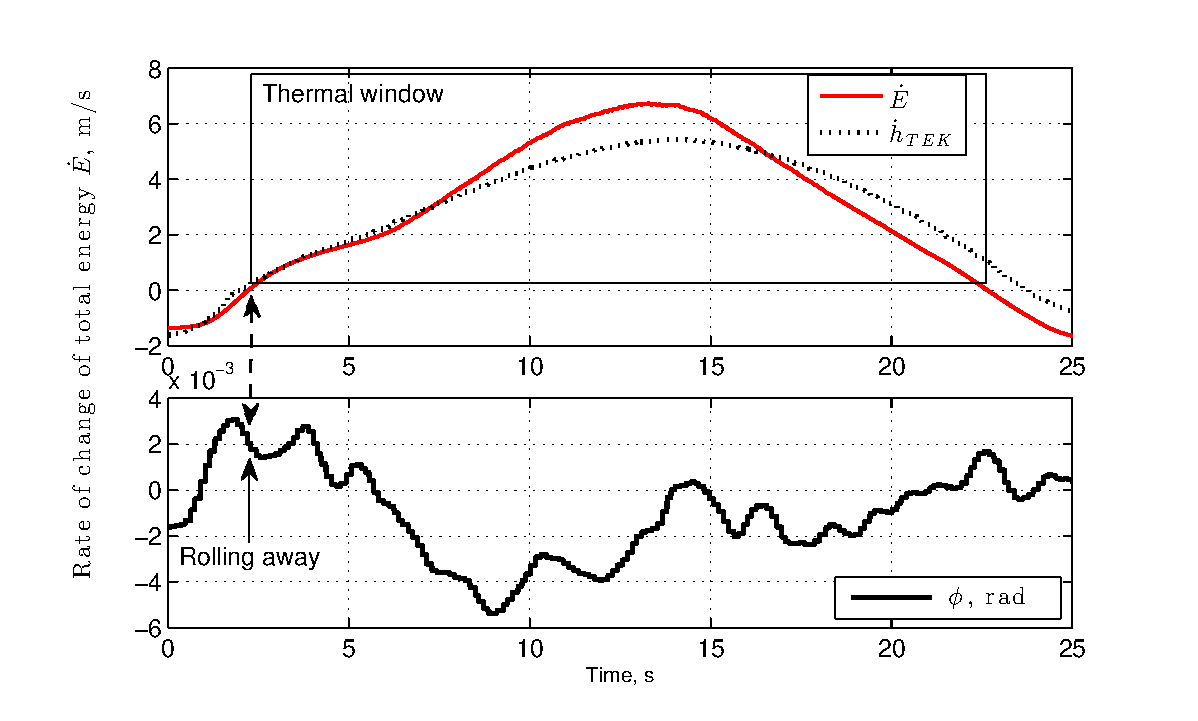
\includegraphics[scale=0.4]{Figures/TEK_Bank.eps}
  \caption{Energy-based detection of updrafts simulated by the software~\cite{Condor:2013:Online}.}
  \label{fig:ThermalDetection}
\end{figure}
%%%%%%%%%%%%%%%%

When a thermal updraft is detected, the glider needs to automatically maneuver to enable staying in the thermal with the objective of increasing the glider's potential energy through a rapid increase of the height. The thermal centering guidance law produces a turn rate command $\dot{\psi}_{c}$ to the autopilot, and is based on the feedback control law that takes into account the desire to get closer to the updraft center (defined by the $\rho_d$), where its intensity (the positive vertical speed) is the highest. On the other hand, the control balances the height increase and the turn-induced sink by a measure proportional to the rate of increase of the total energy (defined by the $\ddot{E}$ in (\ref{eq:totenergyrate})), see the geometry of the guidance task in Figure.\ref{fig:ThermaG} and the resulting guidance law in (\ref{eq:GuidanceLaw}):
\begin{eqnarray}
    && \dot{\psi}_{c}=\frac{V}{\rho_d}-k_1 \cdot \ddot{E},
    \label{eq:GuidanceLaw}
\end{eqnarray}
where $\rho$ and $\rho_d$ are the current distance and the desired orbital radius around the center of the thermal updraft, and $k_1$ is the feedback gain determined by the stability and performance requirements.
%%%%%%%%%%%%%%%%%%%%%%%%%
\begin{figure}[thpb]
  \centering
  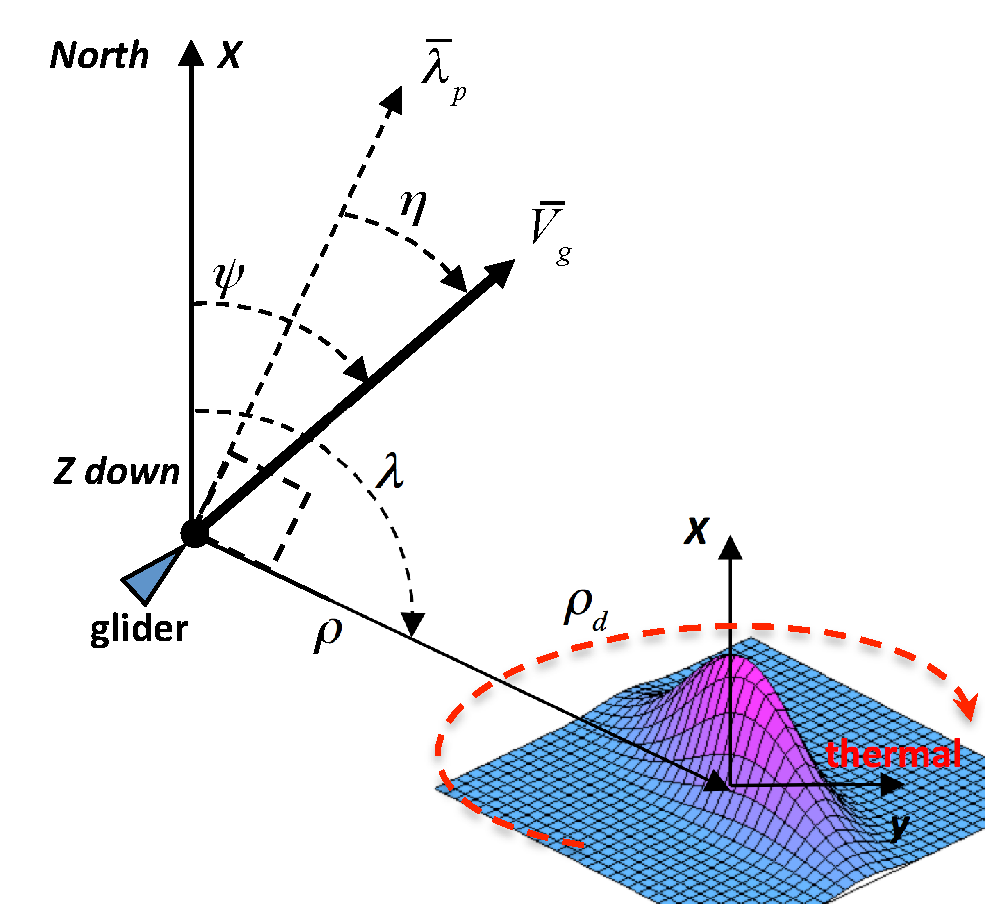
\includegraphics[scale=0.25]{Figures/ThermalG.eps}
  \caption{Kinematics of guidance around a stationary thermal updraft;
  the desired orbit is represented by the red dashed line defined by $\rho_d$.}
  \label{fig:ThermaG}
\end{figure}
%%%%%%%%%%%%%%%%%%%%%%%%%
The physical meaning of the guidance law (\ref{eq:GuidanceLaw}) is to increase the commanded turn rate until the rate of climb in the latched updraft is compensated by the sink resulted from the steep banking; most traditional autopilots implement bank-to-turn control laws.

The initial approach to the estimation of thermals ($2D$ coordinates of the center vs. the glider altitude) by utilizing the measurements of single glider in soaring mode was based on two classical nonlinear filtering techniques: first - the nonlinear Kalman filter with the ''bearings only measurements``, and second - the kinematic relation $\dot{\rho}=-V_g\cdot sin(\eta)$ between the speed over ground $V_g$ and the ''navigation error`` $\eta$, see Figure.\ref{fig:ThermaG}. In both formulations the bearing to the updraft center was assumed to be constant at $\pi/2$ ($\lambda-\psi=\pi/2$) with respect to the direction of turning flight; the turn is defined toward the center of the updraft. When entering a strong updraft, the performance of either filter was slow but reasonable, resulting in a converging solution in about 2 full orbits and precision of the thermal center estimation of $~75m$.

To further improve the efficiency of updraft estimation the solution should integrate the knowledge gained by multiple gliders and the prior meteorological observations, see \cite{Pennycuick:1998,Hindman:2007}), which might be available for the area of operation. The latter data can be conveniently interpreted as a map of probability density of convective air activity with respect to the geographic latitude and longitude, see a conceptual example in Figure.\ref{fig:HeatMap}.
%%%%%%%%%%
\begin{figure}[thpb]
  \centering
  \includegraphics[scale=0.3]{Figures/ProbabilityThermal.eps}
  \caption{The ''heat map`` as a probability density function.}
  \label{fig:HeatMap}
\end{figure}
%%%%%%%%%%
As a first step toward cooperative identification and mapping of convective thermals over extended areas with an account of prior methodological observation, the probabilistic recursive Bayesian approach was adopted, see details of the approach in \cite{Bergman:1999}.

An example of the Bayesian approach for the case of three simulated gliders cooperatively flying and estimating parameters of a single stationary updraft in a given area modeled by a Gaussian model is presented in Figure.\ref{fig:SimPDF}; note, there is no horizontal component of airflow in the model.
%%%%%%%%%%
\begin{figure}[thpb]
  \centering
  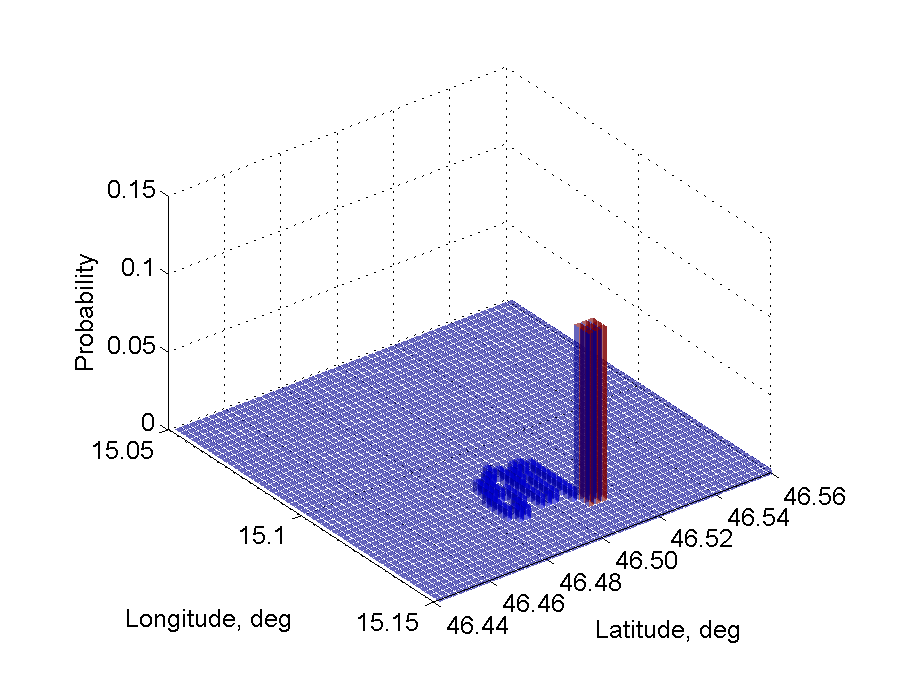
\includegraphics[scale=0.51]{Figures/Mapping_thermals.eps}
  \caption{Estimation of an updraft obtained onboard of glider $\#1$ from
  the cooperative sampling of environment.}
  \label{fig:SimPDF}
\end{figure}
%%%%%%%%%%
\begin{figure}[thpb]
  \centering
  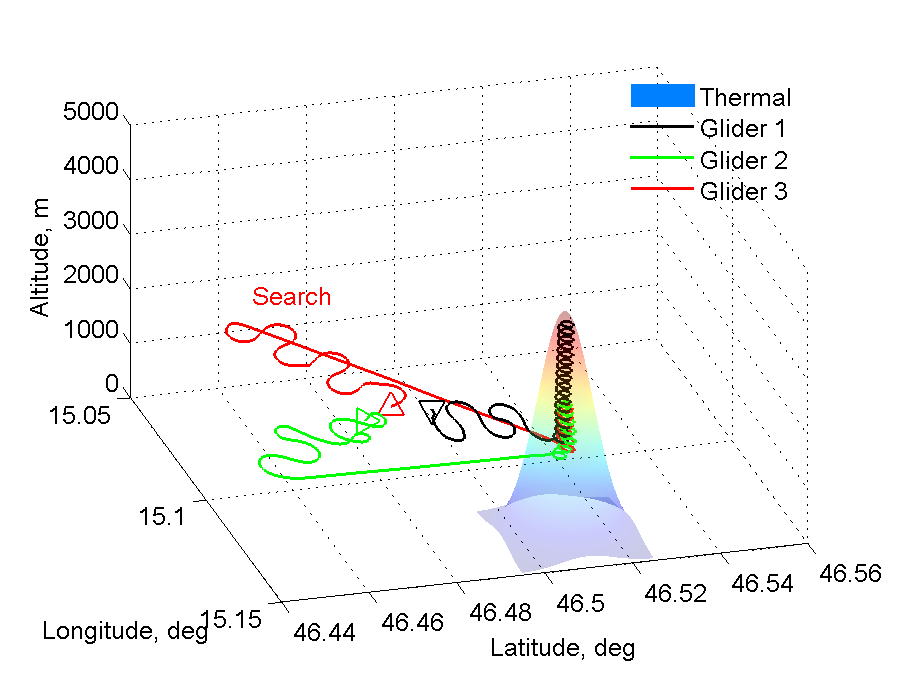
\includegraphics[scale=0.41]{Figures/paths_cooperative_flight.eps}
  \caption{Cooperative flight of three gliders.}
  \label{fig:CoopFlightPaths}
\end{figure}
%%%%%%%%%%
The task is to find the updraft in a bounded area and to converge to the same thermal by utilizing the detection algorithms discussed above; the task mimics the setup and the objectives of the first cooperative flight test of two gliders reported earlier in \cite{AKlass_JGCD:2012}. In the demonstrated
result the prior probability density is initialized by a uniform function over the entire area of operation. The result corresponds to the progression of the probability density function estimated onboard of glider $\#1$ along its flight path, see the corresponding cooperative trajectories of gliders
$\#2$ and $\#3$ in Figure.\ref{fig:CoopFlightPaths}. The gliders start their flight simultaneously at the same altitude, and initially spend some time in search for thermals. When glider $\#1$ detects an updraft utilizing either of the thermal detection approaches and shares the information about the thermal, the other two gliders arrive to the same thermal, and successfully gain height all together. The time history of the altitude gain is presented next in Figure.\ref{fig:CoopFlightHeight}.
%%%%%%%%%%
\begin{figure}[thpb]
  \centering
  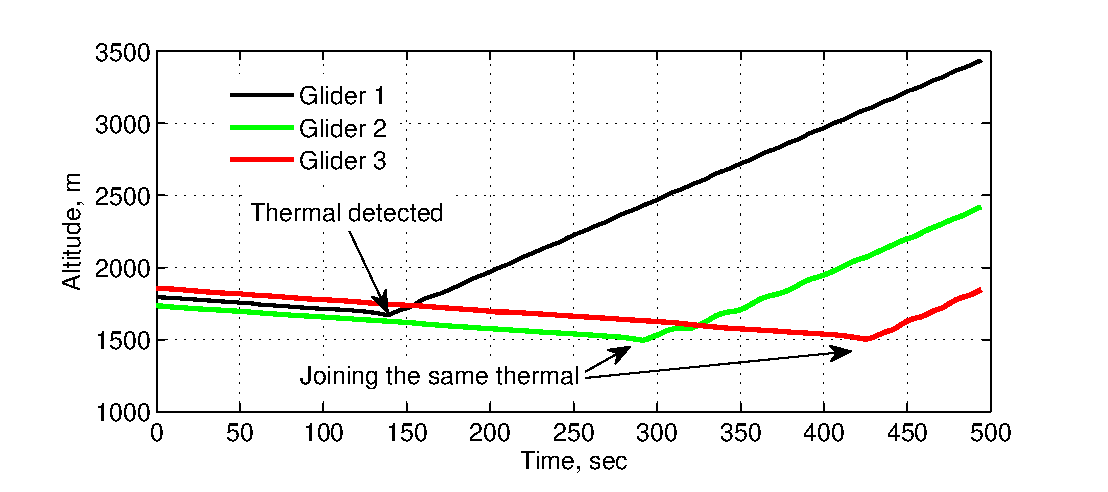
\includegraphics[scale=0.36]{Figures/Coop_gain_altitude.eps}
  \caption{Cooperative gain of altitude.}
  \label{fig:CoopFlightHeight}
\end{figure}
%%%%%%%%%%
\squeezeup
The following result illustrates the capabilities of gliders to make independent decisions in gaining the altitude. The initial settings, the setup, and the goal remain the same. Figure.\ref{fig:CoopFlightIndependentDecision} illustrates that independent decision making allows to utilize the thermals of opportunity by sharing their geographic location and strength found by other gliders. The decision to stay in a newly found thermal is made if its strength is comparable with the strength of nearby ``known'' thermal. The obvious gain of height confirms the efficiency of this strategy.
%%%%%%%%%%
\begin{figure}[thpb]
  \centering
  \includegraphics[scale=0.42]{Figures/SecondExp/paths_cooperative_flight_mod.eps}
  \caption{Independent decision making.}
  \label{fig:CoopFlightIndependentDecision}
\end{figure}
%%%%%%%%%%%
%\squeezeup
%%%%%%%%%%%
%\begin{figure}[thpb]
%  \centering
%  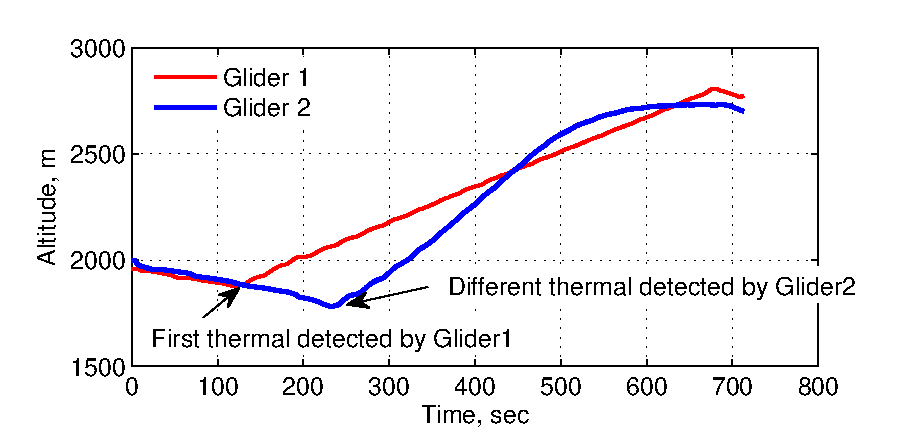
\includegraphics[scale=0.39]{Figures/SecondExp/Thermal_detection_and_gain_altitude_mod.eps}
%  \caption{Independent gain of altitude.}
%  \label{fig:CoopFlightHeightIndependentDecision}
%\end{figure}
%%%%%%%%%%%
The results clearly demonstrate the benefits of collaborative strategies in harvesting the convective updraft energy from the environment.

\section*{CONCLUSIONS}
The paper presents the development of autonomous convective thermal soaring capability of multiple cooperative gliders.
%The discussion details the key technologies required to integrate
%the convective air energy harvesting into a cooperative mission planning and execution environment.
The discussion focuses on the software architecture that allows to design the intelligent cooperative soaring autonomy, and to verify the designed control algorithms in a high-fidelity simulation prior to the actual flight. The key benefits of the software include the ability to realistically represent the atmospheric convective airflow and its interaction with 3D terrain, the high-fidelity flight dynamics of a variety of soaring gliders, and the advance MathWorks' tools of the control development and flight data analysis. The key technologies developed and verified in the novel SIL environment include the online characterization of the inherent flight dynamics of soaring gliders, the convective thermals detection, and the collaborative environment sensing by utilizing recursive Bayesian estimation. Ultimately, the developed system allows V\&V of advanced cooperative control strategies and their comparison against the best practices of human piloted soaring flight.

%%%%%%%%%%%%%%%%%%%%%%%%%%%%%%%%%%%%%%%%%%%%%%%%%%%%%%%%%%%%%%%%%%%%%%%%%%%%%%%%

\bibliographystyle{IEEEtran}
\bibliography{IEEEabrv,iros}

\end{document} 